\documentclass[12pt]{report}
\usepackage[left=2.5cm,right=2.5cm,top=3cm,bottom=3cm]{geometry}
\usepackage{fancyhdr}
\usepackage{etoolbox}
\usepackage{titlesec}
\usepackage{titling} % Para personalizar el título
\usepackage{graphicx}
\usepackage{hyperref}
\usepackage{amsmath}

\geometry{a4paper}

% Configuración de cabecera y pie de página
\pagestyle{fancy}
\fancyhf{} 
\fancyhead[L]{UTN-FRC}
\fancyhead[C]{FÍSICA 2: TPL2}
\fancyhead[R]{2R3}
\renewcommand{\headrulewidth}{0.4pt}
\fancyfoot[C]{\vfill\thepage}

% Cambio en el estilo de las páginas de capítulo
\patchcmd{\chapter}{\thispagestyle{plain}}{\thispagestyle{fancy}}{}{}

% Tamaños de fuente para matemáticas
\DeclareMathSizes{12}{13}{6}{5}

% Configuración del título del documento
\title{%
  \fontsize{25}{0}\selectfont Universidad Tecnológica Nacional \\
  \fontsize{22}{30}\selectfont Física 2 \\
  \fontsize{18}{25}\selectfont TPL2: Capacitores
}
\author{
  Franco Palombo - 401910\\
  Gaston Grasso - 401892\\
  Ignacio Gil - 401891\\
  Santino Noccetti - 405947\\
}
\date{05 / 06 / 2024}

% Formato de títulos y secciones
\titleformat{\chapter}[block]
  {\normalfont\huge\bfseries}{}{0pt}{\Huge}
\titlespacing*{\chapter}{0pt}{-30pt}{20pt}

\titleformat{\section}[block]
  {\normalfont\Large\bfseries}{}{0pt}{\Large}
\titlespacing*{\section}{0pt}{3.5ex plus 1ex minus .2ex}{2.3ex plus .2ex}

\titleformat{\subsection}[block]
  {\normalfont\large\bfseries}{}{0pt}{\large}
\titlespacing*{\subsection}{0pt}{3.25ex plus 1ex minus .2ex}{1.5ex plus .2ex}

\begin{document}
\maketitle

\section{Introducción 1: El Capacitor Plano}

\begin{enumerate}
    \item Al aumentar la diferencia de potencial entre las placas, ¿Qué sucede con la carga de la placa positiva del capacitor? ¿y con la capacidad?\\[6pt]
    Cuando se aumenta la diferencia del potencial del circuito, ambas placas que empiezan teniendo carga neutra empiezan a adquirir una carga negativa y positiva respectivamente, como hay una diferencia de potencial los electrones empiezan a moverse en un cierto sentido, en el caso de la placa que esta mas cercana a la terminal positiva de la bateria, los electrones de la misma van a moverse en direccion de la otra placa  dejando "huecos" o cargandola positivamente mientras que la otra esta siendo invadida por los electrones termina cargandose negativamente.\\
    Como lo unico que varia en esta situacion es la diferencia de potencial, la capacidad no varia ya que depende del area de las placas y la distancia entre las mismas.\\

    
      \begin{figure}[h]
          \centering
          \begin{minipage}[h]{0.45\textwidth}
          \centering
          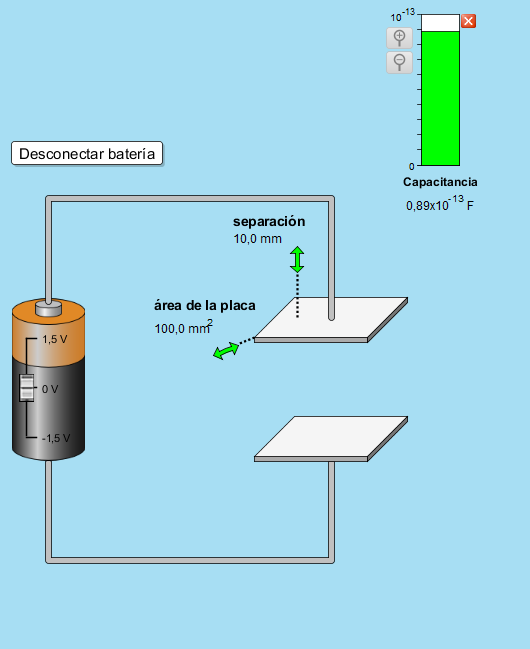
\includegraphics[width=1\textwidth]{./images/1FOTO1.png}
          \textit{Simulacion con las placas sin diferencia de potencial.} 
          \end{minipage}\hskip 1cm
          \begin{minipage}[h]{0.45\textwidth}
          \centering
          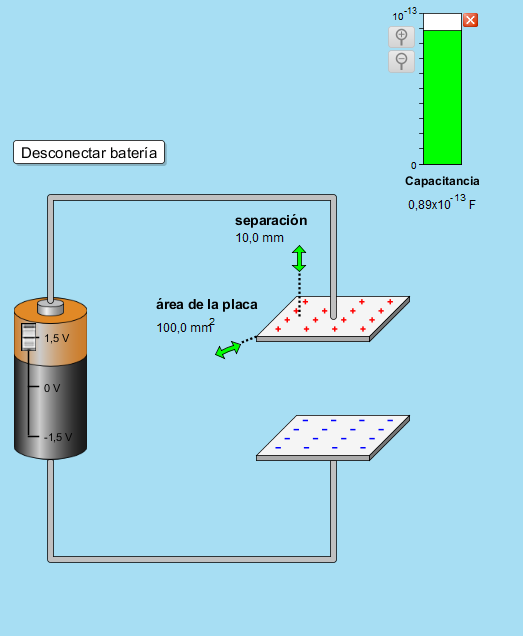
\includegraphics[width=1\textwidth]{./images/1FOTO2.png}
          \textit{Simulacion con las placas con diferencia de potencial.} 
       \end{minipage}
      \end{figure}

\newpage

    \item Fijá la diferencia de potencial a 1,5 V, habilitá el voltímetro y explica qué sucede con la carga, con la diferencia de potencial y con la capacidad, al variar el área de las placas.\\[6pt]
    Si se conecta la bateria con un voltaje de 1.5 V y mido entre las placas, me va a mostrar el mismo valor que la fuente, si a las placas les aumento el area entonces se va a lograr que: un incremento en la capacidad de la cantidad de cargas que puedan contener, esto conlleva a un aumento de capacitancia, pero esto no implica a una variacion de diferencia de potencial ya que ambas placas estan conectadas a la fuente por lo que el voltimetro va a seguir mostrando el mismo valor.

    Para que el voltaje se mantenga  constante significa que la carga de las placas deban aumentar  proporcionalmente al area de las mismas.

Lo anterior se puede comprobar con la siguiente formula de capacitancia y de diferencia de potencial entre las placas:
    \begin{center}
    \[C=e_0\frac{A}{d}\]
    \[V_{ab}=\frac{Qd}{\epsilon_0A}\]
    \end{center}

    \begin{figure}[h]
        \centering
        \begin{minipage}[h]{0.45\textwidth}
        \centering
        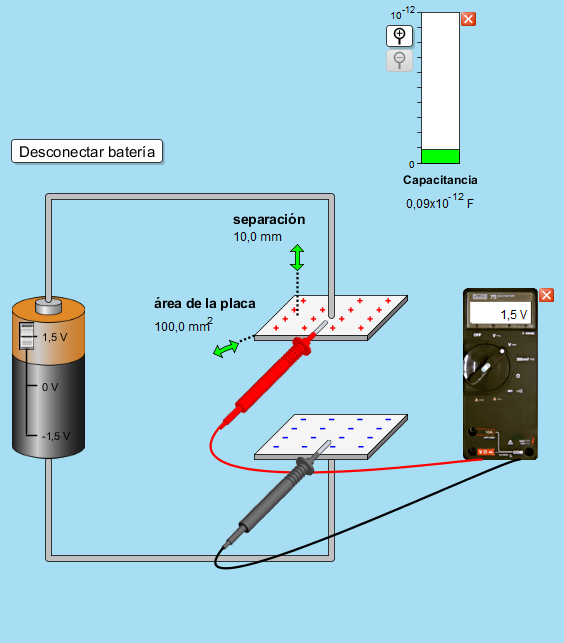
\includegraphics[width=1\textwidth]{./images/1FOTO3.png}
        \textit{Simulacion con area de \(100mm^2\).} 
        \end{minipage}\hskip 1cm
        \begin{minipage}[h]{0.45\textwidth}
        \centering
        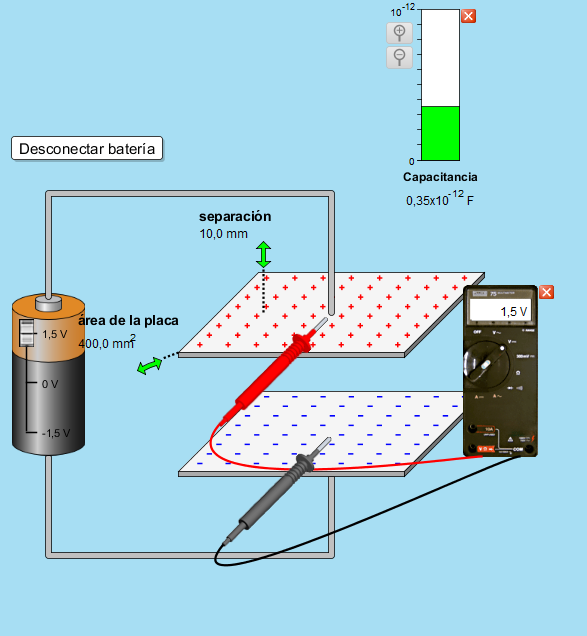
\includegraphics[width=1\textwidth]{./images/1FOTO4.png}
        \textit{Simulacion con area de \(400mm^2\).} 
     \end{minipage}
    \end{figure}

\newpage

    \item Modificá el espacio entre las placas y comenta qué sucede con la carga, la capacidad y la diferencia de potencial.\\[6pt]
    En el caso de que se varie unicamente la distancia entre las placas, la capacidad obtiene una variacion inversamente proporcional y se ve un aumento de determinadas cargas en cada placa. En este caso como se tiene la fuente conectada no va a haber una variacion de diferencia de potencial cuando disminuya la distancia, ya que va a haber un aumento en las cargas de cada placa por el incremento de atraccion de las mismas.

Esto se puede ver con las mismas formulas del enunciado anterior.\\

    \begin{figure}[h]
        \centering
        \begin{minipage}[h]{0.45\textwidth}
        \centering
        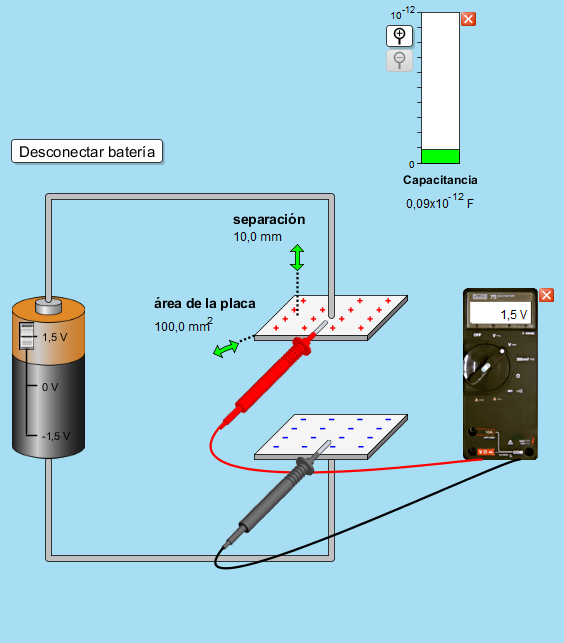
\includegraphics[width=1\textwidth]{./images/1FOTO5.png}
        \textit{Simulacion con distancia de 10mm.} 
        \end{minipage}\hskip 1cm
        \begin{minipage}[h]{0.45\textwidth}
        \centering
        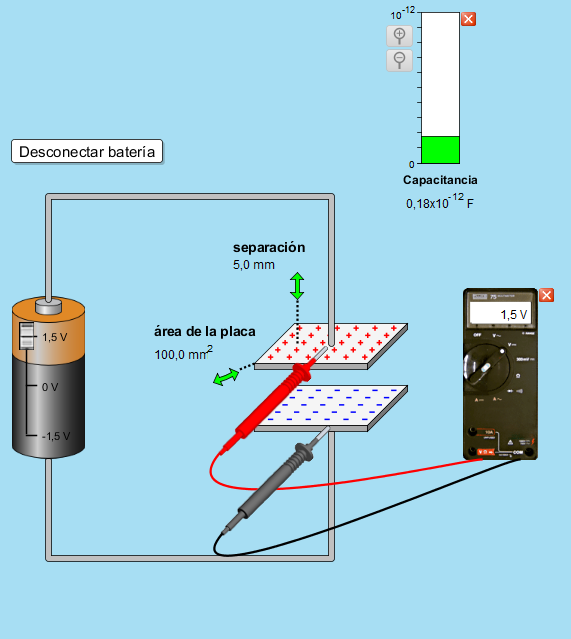
\includegraphics[width=1\textwidth]{./images/1FOTO6.png}
        \textit{Simulacion con distancia de 5mm.} 
     \end{minipage}
    \end{figure}

\end{enumerate}

\newpage

\section{Introducción 2: El Campo Eléctrico}

Habilitá el detector de campo eléctrico, y manteniendo la pila conectada responde a las siguientes preguntas:\\[6pt]
\begin{enumerate}
    \item ¿Qué sucede con la intensidad del campo eléctrico al variar el área de las placas? ¿Podrías explicar por qué?\\[6pt]
    Cuando varie el area de las placas con la fuente conectada no va a haber una variacion de la intensidad del campo electrico. Debido a que el voltaje permanece constante por estar conectado a la bateria, segun la ecuacion de diferencia de potencial para capacitores de placas paralelas en vacio:

    \[V_{ab}=\vec{E} \cdot \vec{d}\]

    Ambas magnitudes tienen que permanecer constantes para que la diferencia de potencial siga siendo la misma siendo esta dictada por la bateria. Debido a que la distancia permanece constante centramos nuestro analisis en la formula de capacitores de placas paralelas en vacio, definido como:

    \[\vec{E}=\frac{\sigma}{\epsilon_0}=\frac{Q}{\epsilon_0 A}\]

    Al variar el area la unica forma de que el campo electrico permanezca constante es aumentando adecuadamente la carga. Ese aumento en la carga produce que la capacitancia aumente por la formula de capacitancia de capacitores:

    \[C=\frac{Q}{V_{ab}}\]

    \begin{figure}[h]
        \centering
        \begin{minipage}[h]{0.4\textwidth}
        \centering
        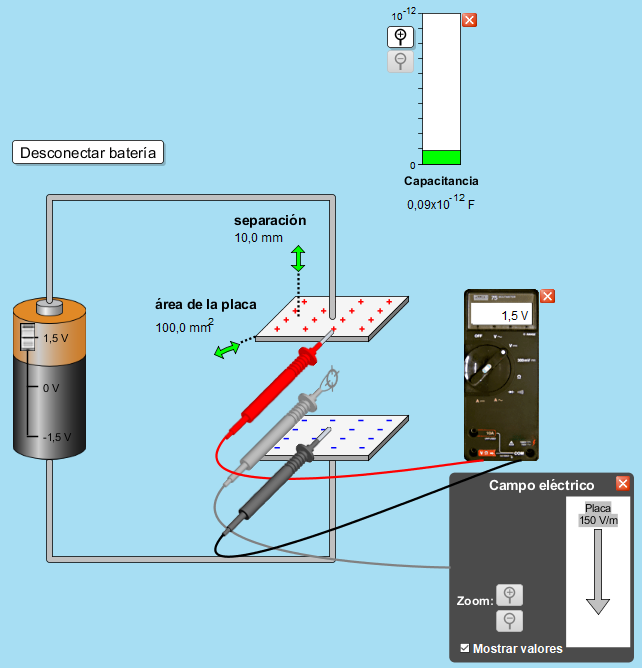
\includegraphics[width=1\textwidth]{./images/2FOTO1.png}
        \textit{Simulacion con area inicial.} 
        \end{minipage}\hskip 1cm
        \begin{minipage}[h]{0.4\textwidth}
        \centering
        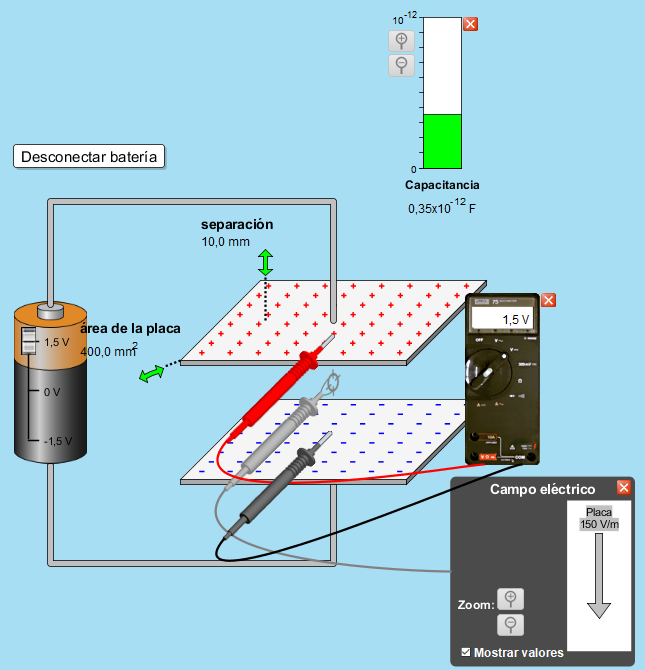
\includegraphics[width=1\textwidth]{./images/2FOTO2.png}
        \textit{Simulacion con area final.} 
     \end{minipage}
    \end{figure}

\newpage

    \item ¿Qué sucede con la intensidad del campo al variar el espaciamiento entre las placas? ¿A qué se debe?\\[6pt]
    Como se vio previamente, si yo hago variar la distancia entre ambas placas en vacio estando conectado en la fuente, se logra un incremento de cargas en las placas para que la diferencia de potencial se mantenga constante. El resultado de esto se ve afectado en el incremento del flujo, por ende, tambien hay un aumento del campo electrico inversamente proporcional a la variacion de la distancia.

    \begin{figure}[h]
        \centering
        \begin{minipage}[h]{0.4\textwidth}
        \centering
        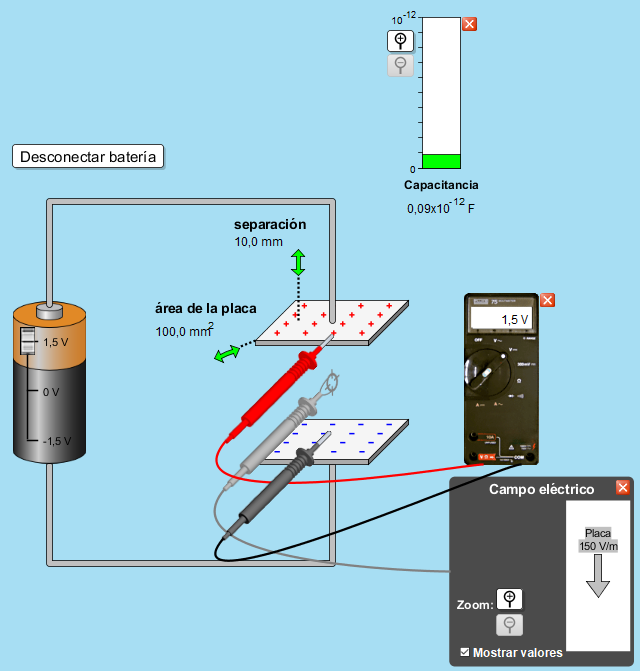
\includegraphics[width=1\textwidth]{./images/2FOTO3.png}
        \textit{Simulacion con distancia inicial.} 
        \end{minipage}\hskip 1cm
        \begin{minipage}[h]{0.4\textwidth}
        \centering
        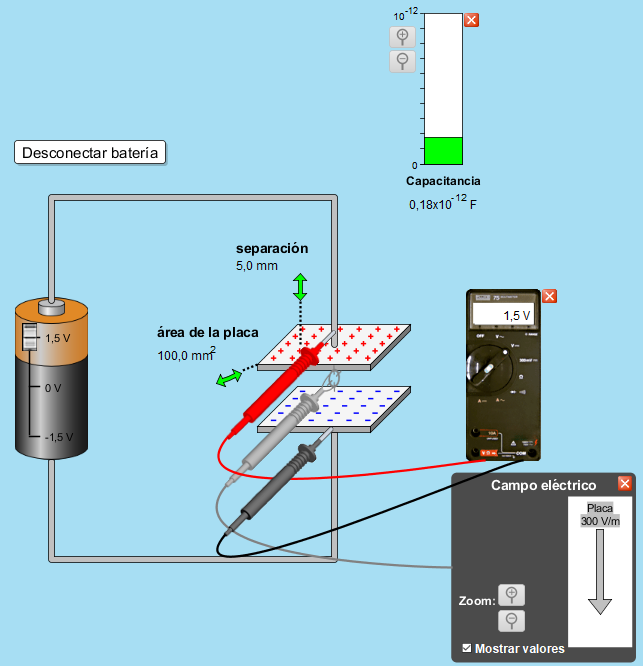
\includegraphics[width=1\textwidth]{./images/2FOTO4.png}
        \textit{Simulacion con distancia final.} 
     \end{minipage}
    \end{figure}
\end{enumerate}

\newpage 

\section{Desconexión de la Fuente}

\begin{enumerate}
    \item Fijá la tensión de la fuente a 1,5 V, la separación de las placas en 10 mm y el área a 100 mm$^2$. Mantené el voltímetro y el sensor de campo eléctrico conectados y luego desconectá la fuente.
    \begin{enumerate}
        \item ¿Qué sucede con la carga, diferencia de potencial, capacidad e intensidad del campo eléctrico al disminuir el espaciamiento entre las placas?\\[6pt]
            Al disminuir la distancia entre las placas, la diferencia de potencial del capacitor disminuye, mientras que la capacidad del mismo aumenta. En cambio, la carga  y el campo eléctrico permanecen constantes.
        
      \begin{figure}[h]
          \centering
          \begin{minipage}[h]{0.4\textwidth}
          \centering
          \includegraphics[width=1\textwidth]{./images/3foto1.jpg}
          \textit{Capacitor original.} 
          \end{minipage}\hskip 1cm
          \begin{minipage}[h]{0.4\textwidth}
          \centering
          \includegraphics[width=1\textwidth]{./images/3foto2.jpg}
          \textit{Capacitor alterado.} 
       \end{minipage}
      \end{figure}

        
  \item ¿Qué sucede con la carga, diferencia de potencial, capacidad e intensidad de campo eléctrico al aumentar el área de las placas?\\[6pt]
            Al aumentar el área de las placas, la diferencia de potencial disminuye considerablemente, al igual que el campo entre las placas, mientras que la capacidad aumenta considerablemente. La carga permanece constante.\\

      \begin{figure}[h]
          \centering
          \begin{minipage}[h]{0.4\textwidth}
          \centering
          \includegraphics[width=1\textwidth]{./images/3foto1.jpg} 
          \textit{Capacitor original.} 
          \end{minipage}\hskip 1cm
          \begin{minipage}[h]{0.4\textwidth}
          \centering
          \includegraphics[width=1\textwidth]{./images/3foto3.jpg} 
          \textit{Capacitor alterado.} 
       \end{minipage}
      \end{figure}

            \vspace{10cm}

        
    \end{enumerate}
    \item Conecta nuevamente el capacitor a la fuente de 1,5 V, fijá la separación de las placas a 5 mm, y el área a 400 mm$^2$. Ahora desconecta el capacitor de la fuente y responde:
    \begin{enumerate}
        \item ¿Qué sucede con la carga, diferencia de potencial, capacidad e intensidad de campo eléctrico al aumentar el espaciamiento entre las placas?\\[6pt]
        Al aumentar la distancia entre las placas, la diferencia de potencial del capacitor aumenta, mientras que la capacidad del mismo disminuye. En cambio, la carga  y el campo eléctrico permanecen constantes.\\

      \begin{figure}[h]
          \centering
          \begin{minipage}[h]{0.4\textwidth}
          \centering
          \includegraphics[width=1\textwidth]{./images/3foto4.jpg} 
          \textit{Capacitor original.} 
          \end{minipage}\hskip 1cm
          \begin{minipage}[h]{0.4\textwidth}
          \centering
          \includegraphics[width=1\textwidth]{./images/3foto5.jpg} 
          \textit{Capacitor alterado.} 
       \end{minipage}
      \end{figure}

        
  \item ¿Qué sucede con la carga, diferencia de potencial, capacidad e intensidad de campo eléctrico al disminuir el área entre las placas?\\[6pt]
            Al disminuir el área de las placas, la diferencia de potencial aumenta considerablemente, al igual que el campo entre las placas, mientras que la capacidad disminuye considerablemente. La carga permanece constante.\\

      \begin{figure}[h]
          \centering
          \begin{minipage}[h]{0.4\textwidth}
          \centering
          \includegraphics[width=1\textwidth]{./images/3foto4.jpg} 
          \textit{Capacitor original.} 
          \end{minipage}\hskip 1cm
          \begin{minipage}[h]{0.4\textwidth}
          \centering
          \includegraphics[width=1\textwidth]{./images/3foto6.jpg} 
          \textit{Capacitor alterado.} 
       \end{minipage}
      \end{figure}
        
\newpage

    \end{enumerate}
    \item ¿Podrías explicar lo sucedido en 1 y en 2?\\[6pt] 
    Para todos los casos, la carga permanece constante debido a que el capacitor, permanece "en vacío" para todas las pruebas. Esto implica que no hay movimiento de cargas en ningún momento.

    Para todos los casos, la variación de capacidad está dictada por la fórmula de capacitancia:

\[C=\frac{Q}{V_{ab}}\]

    Debido a que la carga del capacitor permanece siempre constante, el único parámetro que puede alterar la capacidad es la diferencia de potencial, que, como se vio antes, varía en todos los casos.
    
    La diferencia de potencial, se puede definir como:
    
\[V_a-V_b=\int_{a}^{b}\vec{E}\cdot d \vec{l}\]

    Cuando variamos la distancia entre las placas, el campo eléctrico permanece constante, por lo que la variación está dictada por \(d \vec{l}\). La variación de la distancia es directamente proporcional a la diferencia de potencial entre las placas. Mientras más chica sea la distancia, menor el voltaje, y mientras más grande, mayor el voltaje.

    Ahora, para los casos en los que el campo eléctrico varía, la distancia entre las placas permanece constante. Podemos definir el campo eléctrico para un capacitor de placas paralelas en vacio como:
    
\[\vec{E}=\frac{\sigma}{\epsilon_0}=\frac{Q}{\epsilon_0 A}\]

    El aumento en el área tiene un efecto inverso en el campo eléctrico. Esto es porque al mantenerse las cargas constantes, si aumentamos el área disminuye drásticamente la densidad de carga por unidad de área. En cambio, si se disminuye el área, las cargas son las mismas pero se tienen que acomodar en una superficie más chica que antes, por lo que la densidad de carga aumenta drásticamente.

\end{enumerate}

\newpage

\section{Introduzcamos un Dieléctrico}

\begin{enumerate}
    \item Seleccioná el aislante dieléctrico que prefieras y, con la fuente conectada, introdúcelo entre las placas del capacitor.
        \\\\Se selecciono como aislante al teflon, que tiene una constante dielectrica $k = 2,1$.

    \begin{enumerate}
        \item ¿Qué cambios se observan en el material? (Puedes tildar la casilla “mostrar cargas en exceso” para ver mejor el fenómeno).\\[6pt]
Al introducir el dielectrico entre las placas, este se polariza. Esto se puede visualizar mostrando las cargas en exceso al ver que las cargas opuestas dentro del dielectrico se trasladan hacia los extremos del material, atrayendose las cargas positivas del dielectrico a las negativas de la placa y las cargas negativas del dielectrico a las positivas de la placa.\\

        \item ¿Cuánto vale el campo eléctrico resultante entre las placas? ¿Cuánto valía el campo eléctrico entre las placas antes de introducir el dieléctrico? ¿Qué puedes decir al respecto?\\[6pt]
El campo electrico resultante entre las placas al introducir el dielectrico vale $150\frac{V}{m}$. Antes de introducir el dielectrico, tambien valia $150\frac{V}{m}$. Esto se debe a que antes de introducirlo, el unico campo que se produce es el que hay entre las placas y que es proporcional a la diferencia de potencial y al area de las placas. Al introducir el dielectrico, el campo entre las placas aumenta ya que al introducir el dielectrico, la capacitancia aumenta y si mantenemos el voltaje constante, segun $C = \frac{Q}{V}$, la carga debe aumentar, y por ende el campo tambien aumenta a $E_p = 315\frac{V}{m}$; pero hay que tener en cuenta tambien el campo inducido que se le resta, que vale $E_i = 165\frac{V}{m}$, siendo $E_p - E_i = 150\frac{V}{m}$.\\

        \item La simulación te presenta el valor del campo eléctrico inducido, el campo eléctrico en el vacío, y el campo eléctrico resultante. En base a éstos, intenta calcular la constante dieléctrica y verificar el valor proporcionado por el simulador.\\[6pt]
        Para calcular el dielectrico, usamos la formula:
        \[k = \frac{C_f}{C_o}\] donde reemplazamos C
        \[k = \frac{\frac{Q_f}{V}}{\frac{Q_o}{V}}\] Como V es constante, se cancelan y queda:
        \[k = \frac{Q_f}{Q_o}\] Para calcular $Q_f$ y $Q_o$ usamos:
        \[E = \frac{Q}{\epsilon_o \cdot A}\]
        \begin{align*}
          Q_f&= \epsilon_o \cdot A \cdot E_i                           & Q_o&=\epsilon_o \cdot A \cdot E_i\\[6pt]
          Q_f&= \epsilon_o \cdot 0,0001 m^2 \cdot 315 \frac{V}{m}      &Q_o&= \epsilon_o \cdot 0,0001 m^2 \cdot 150 \frac{V}{m}\\[6pt]
          Q_f&= 0,279 \cdot 10^{-12} C                                  &Q_o&= 0,133 \cdot 10^{-12} C\\[6pt]
        \end{align*}
        Entonces:

        \begin{align*}
          k&= \frac{0,279 \cdot 10^{-12} C }{0,133 \cdot 10^{-12} C}\\[6pt]
          k&= 2,1\\[6pt]
        \end{align*}

        Este resultado es igual al que nos indica la simulación.

        \item ¿Qué sucede con las cargas en las placas metálicas, la diferencia de potencial, la capacidad cuando se introduce el dieléctrico?\\[6pt]
        Las cargas aumentan, la diferencia de potencial es constante y la capacidad tambien aumenta. Como se dijo anteriormente, esto esta dado por:
        \[C = \frac{Q}{V}\]

        \item Habilita la casilla de “Energía almacenada” y cuéntame qué ocurre con la energía al introducir un dieléctrico. Realiza el cociente entre la energía almacenada con dieléctrico y la almacenada sin dieléctrico. Compara dicho cociente con la constante dieléctrica.\\[6pt]
        La energia almacenada aumenta al introducir el dielectrico. Si evaluamos el cociente:
        \begin{align*}
          k &= \frac{E_f}{E_o}\\[6pt]
          k &= \frac{0,21 \cdot 10^{-12} J}{0,1 \cdot 10^{-12} J}\\[6pt]
          k &= 2,1
        \end{align*}

        Se puede ver que también es igual al que nos proporciona la simulacion.

    \end{enumerate}
    \item Ahora, retira el dieléctrico y asegúrate que la pila aporte una diferencia de potencial de 1,5 V. Luego, desconecta la fuente y vuelve a introducir el dieléctrico.
    \begin{enumerate}
        \item ¿Cuánto vale el campo eléctrico resultante entre las placas? ¿Y entre las placas cuando no hay material? ¿Qué puedes decir al respecto?\\[6pt]
        El campo electrico resultante vale $71 \frac{V}{m}$ cuando hay material y $150 \frac{V}{m}$ cuando no hay material. Esto se debe a que el Campo Electrico entre las placas es constante, ya que al desconectar la bateria, el capacitor no tiene donde descargarse. Como al introducir el dielectrico se induce un campo electrico opuesto al que hay entre las placas, se le resta a los $150 \frac{V}{m}$ iniciales.\\

        \item Vuelve a verificar el valor de la constante dieléctrica en base a la intensidad de los campos. ¿Se obtiene el mismo valor que el obtenido con la fuente conectada?\\[6pt]
        Para calcular este valor, se simplificarán los calculos usando la formula $k = \frac{E_f}{E_o}$ debido a que la carga es constante. Luego de hacer el cociente, se verifica que en efecto es el mismo valor que dió anteriormente (2,1).\\

        \item ¿Qué sucede con las cargas en las placas metálicas, la diferencia de potencial, la capacidad cuando se introduce el dieléctrico?\\[6pt]
        Las cargas se mantienen constantes, la diferencia de potencial disminuye y la capacidad aumenta.\\

        \item ¿Qué ocurre con la energía al introducir un dieléctrico? Realiza el cociente entre la energía almacenada con dieléctrico y la almacenada sin dieléctrico. Compara dicho cociente con la constante dieléctrica.\\[6pt]
        La energia disminuye al introducir el dielectrico. Antes de introducirlo vale $0,1 \cdot 10^{-12} J$ y luego de introducirlo vale $0,0476 \cdot 10^{-12} J$. Al realizar el cociente entre los dos, da como resultado 2,1.\\


    \end{enumerate}
\end{enumerate}

\newpage

\section{Conexión de Capacitores}

\begin{enumerate}
    \item Arma un circuito serie de dos capacitores de capacidades $C_1 = 2 \times 10^{-13} \, \text{F}$ y $C_2 = 3 \times 10^{-13} \, \text{F}$ con una batería de 1,5 V.
    \begin{enumerate}
        \item Mide los campos eléctricos de ambos capacitores. ¿Qué relación guardan entre sí?\\[6pt]
            Los campos electricos son iguales, tanto en magnitud como en sentido.\\
        \item Mide la carga de cada capacitor. ¿Qué relación guardan entre sí?\\[6pt]
            Teniendo en cuenta que $Q=C \times V$ 
            \begin{align*}
            Q_1&= C_1 \times V_1\\[6pt]
            Q_1&= 2 \times 10^{-13} \,\text{F} \times 0.9 \text{V}\\[6pt]
            Q_1&= 1.8\times 10^{-13} \,\text{C}
            \end{align*}
            \begin{align*}
            Q_2&= C_2 \times V_2\\[6pt]
            Q_2&= 3 \times 10^{-13} \,\text{F} \times 0.6 \text{V}\\[6pt]
            Q_2&= 1.8\times 10^{-13} \,\text{C}\\[12pt]
            \end{align*}
            La carga en los 2 capacitores es igual\\

        \item Mide las diferencias de potencial entre las placas de cada capacitor. ¿Qué relación guardan con la diferencia de potencial aportada por la batería?\\[6pt]
            La suma de las diferencias de potencial en los capacitores es igual a la diferencia de potencial que entrega la bateria.\\

\newpage

        \item Calcula la capacidad de un supuesto capacitor que acumule la misma carga, y esté sometido a la misma diferencia de potencial total que el conjunto $\{C_1, C_2\}$ (capacitor equivalente).\\[6pt]
            El capacitor equivalente se puede calcular teniendo en cuenta que los 2 capacitores estan dispuestos en serie, entonces:\\

            \begin{align*}
                C_{eq}&= \frac{1}{\frac{1}{C1}+\frac{1}{C2}}\\[6pt]
                C_{eq}&= \frac{1}{\frac{1}{C1}+\frac{1}{C2}}\\[6pt]
                C_{eq}&= \frac{1}{\frac{1}{2 \times 10^{-13} \,\text{F}}+\frac{1}{3 \times 10^{-13} \,\text{F} }}\\[6pt]
                C_{eq}&= 1.2 \times 10^{-13} \,\text{F}\\[12pt]
            \end{align*}

        \item Verifica el cálculo anterior reemplazando ambos capacitores por el equivalente y verificando su carga, campo eléctrico y diferencia de potencial.\\

\begin{figure}[h]
    \centering
    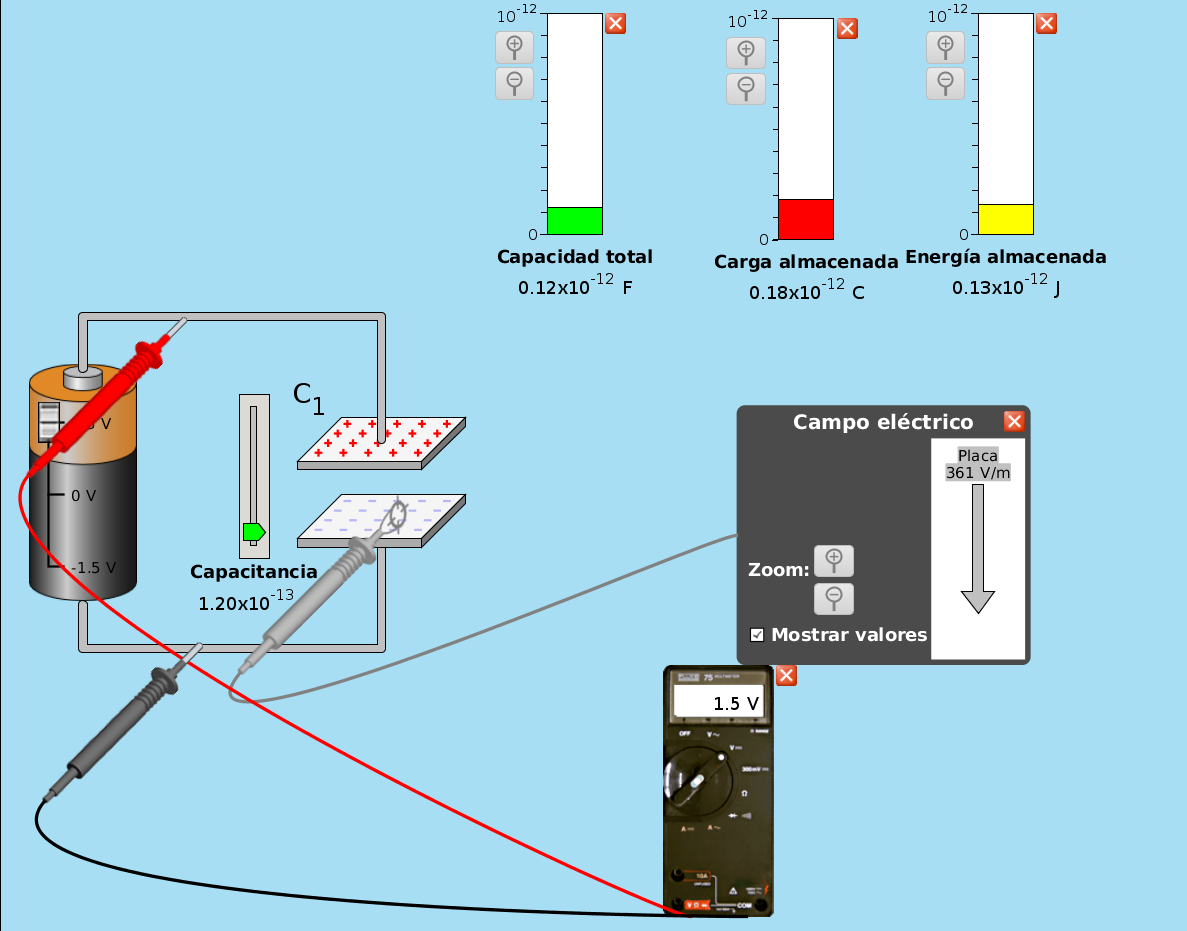
\includegraphics[width=0.9\textwidth]{./images/foto1ejercicio1Conexiondecapacitores.png}
\end{figure}
 
            \vspace{5cm}

    \end{enumerate}
    
    \item Arma un circuito paralelo de dos capacitores de capacidades $C_1 = 1 \times 10^{-13} \, \text{F}$ y $C_2 = 2 \times 10^{-13} \, \text{F}$ con una batería de 1,5 V.
    \begin{enumerate}
        \item Mide los campos eléctricos de ambos capacitores. ¿Qué relación guardan con las capacidades?\\[6pt]
            Los campos electricos de cada capacitor son distintos y directamente proporcionales a la capacitancia de cada uno.\\
        \item Mide la carga de cada capacitor. ¿Qué relación guardan con los campos eléctricos?\\[6pt]
            Teniendo en cuenta que $Q=C \times V$
            
            \begin{align*}
            Q_1&= C_1 \times V_1\\[6pt]
            Q_1&= 1 \times 10^{-13} \,\text{F} \times 1.5 \text{V}\\[6pt]
            Q_1&= 1.5\times 10^{-13} \,\text{C}
            \end{align*}


            \begin{align*}
            Q_2&= C_2 \times V_1\\[6pt]
            Q_2&= 2 \times 10^{-13} \,\text{F} \times 1.5 \text{V}\\[6pt]
            Q_2&= 3\times 10^{-13} \,\text{C}\\[12pt] 
            \end{align*}

            La cara de cada capacitor es proporcional al campo electrico de cada uno, ya que la diferencia de potencial entre las placas de cada uno es igual.\\

        \item Mide las diferencias de potencial entre las placas de cada capacitor. ¿Qué relación guardan con la diferencia de potencial aportada por la batería?\\[6pt]
            La diferencia de potencial entre las placas de cada capacitor es igual por la disposición en paralelo.\\

\newpage

        \item Calcula la capacidad de un capacitor que, sometido a la misma diferencia de potencial, acumule la misma carga total que el conjunto $\{C_1, C_2\}$.\\[6pt]
            El capacitor equivalente de 2 capacitores en paralelo es:\\
            $C_{eq}=C_1+C_2$ Entonces:\\

            \begin{align*}
                C_{eq}&=C_1+C_2\\[6pt]
                C_{eq}&= 1 \times 10^{-13} \, \text{F} +  2 \times 10^{-13} \, \text{F}\\[6pt]
                C_{eq}&= 3\times 10^{-13} \, \text{F}\\[12pt]
            \end{align*}


        \item Verifica el cálculo anterior reemplazando ambos capacitores por el equivalente y verificando su carga, campo eléctrico y diferencia de potencial.

\begin{figure}[h]
    \centering
    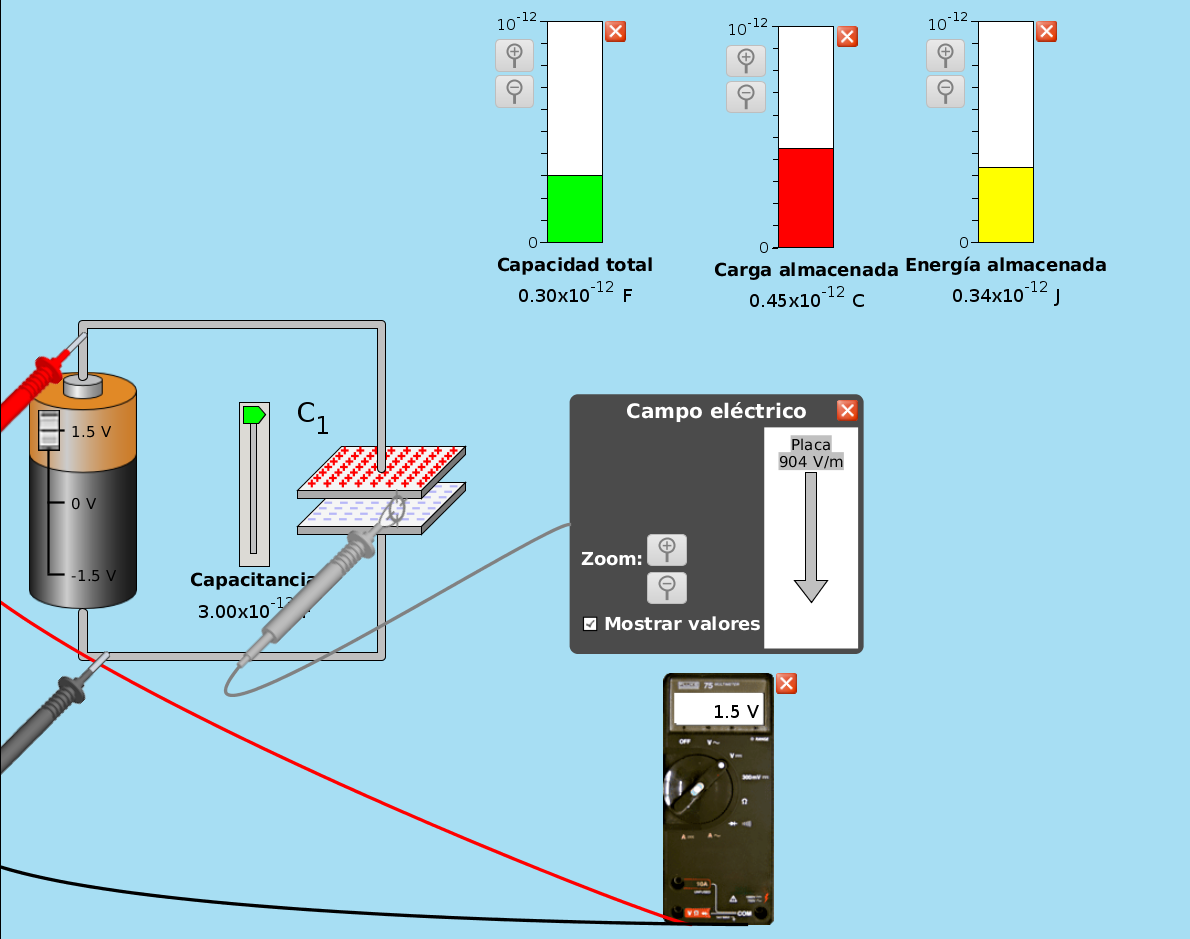
\includegraphics[width=0.9\textwidth]{./images/foto1ejercicio2Conexiondecapacitores.png}
\end{figure}
    \end{enumerate}

    \vspace{10cm}


\item Construye dos circuitos mixtos como los de las siguientes figuras. Luego, mide las diferencias de potencial a los bornes de cada capacitor, el campo eléctrico entre las placas de cada uno, la carga de cada uno y la energía total acumulada. Luego, verifica todas estas cantidades de manera analítica.\\




    \textbf{Circuito 1}\\
    Primero Calculamos el capacitor equivalente, esto es igual a:\\
\begin{align*}
    C_{eq}&=\frac{1}{\frac{1}{C_1}+\frac{1}{C_2+c_3}}\\[6pt]
    C_{eq}&=\frac{1}{\frac{1}{1 \times 10^{-13} \, \text{F} }+\frac{1}{2 \times 10^{-13} \, \text{F}+ 3 \times 10^{-13} \, \text{F}}}\\[6pt]
    C_{eq}&=8.333 \times 10^{-14} \, \text{F}\\[6pt]
\end{align*}

Ahora, la carga total acumulada:\\
\begin{align*}
    Q&=C \times V\\[6pt]
    Q&=8.333 \times 10^{-14} \, \text{F} \times 1.5V \\[6pt]
    Q&=1.25 \times 10^{-13} \, \text{C}\\[6pt]
\end{align*}

Ahora, calculamos la energia total almacenada:\\
\begin{align*}
    E&=\frac{1}{2}\times C\times V^2\\[6pt]
    E&=\frac{1}{2}\times 8.333 \times 10^{-14} \, \text{F} \times 1.5V^2\\[6pt]
    E&= 9.371 \times 10^{-14} \, \text{J}\\[20pt]
\end{align*}

\begin{figure}[h]
    \centering
    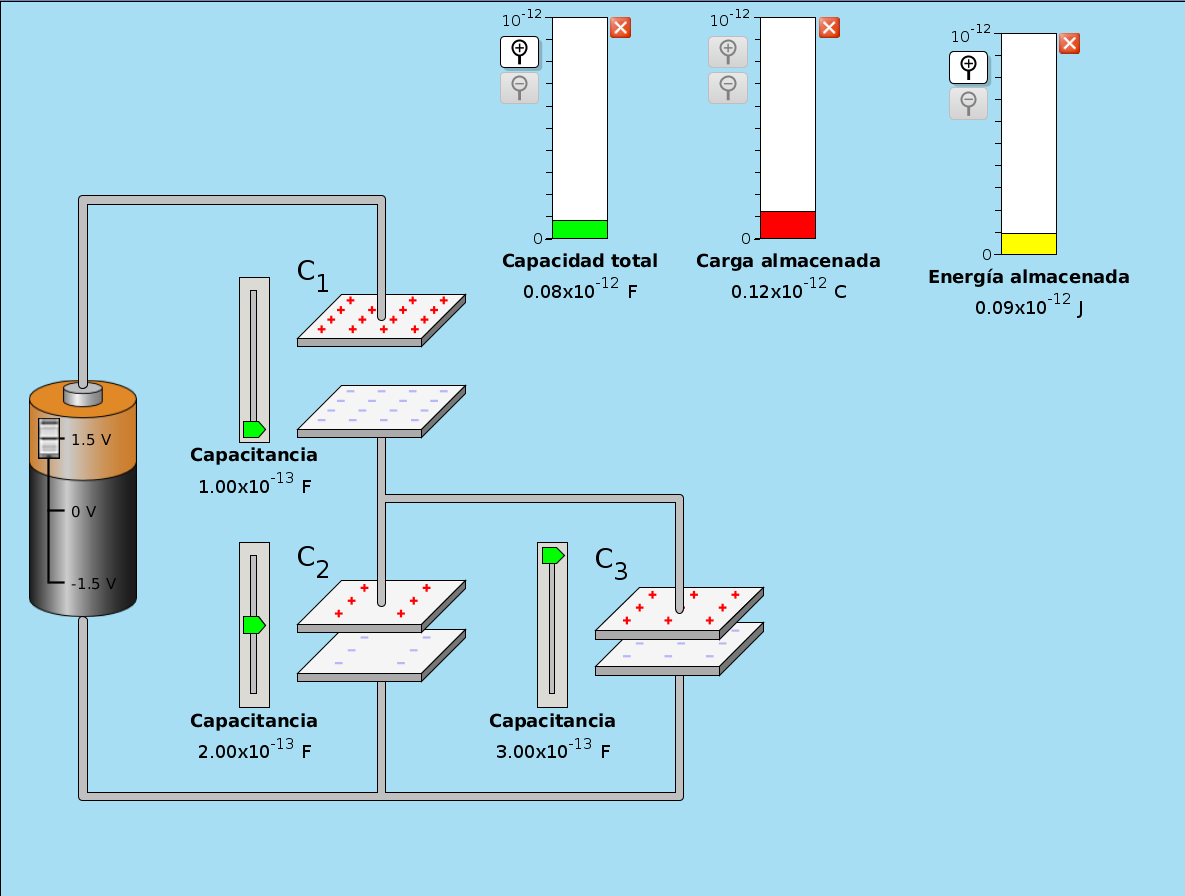
\includegraphics[width=0.9\textwidth]{./images/foto1ejercicio3Conexiondecapacitores.png}
\end{figure}

\vspace{5cm}

    \textbf{Circuito 2}\\
    Primero Calculamos el capacitor equivalente, esto es igual a:\\
\begin{align*}
    C_{eq}&=\frac{1}{\frac{1}{C_1}+\frac{1}{C_2}}+C_3\\[6pt]
    C_{eq}&=\frac{1}{\frac{1}{3 \times 10^{-13} \, \text{F} }+\frac{1}{2 \times 10^{-13} \, \text{F}}}+ 3 \times 10^{-13} \, \text{F}\\[6pt]
    C_{eq}&=2.2 \times 10^{-13} \, \text{F}\\[6pt]
\end{align*}

Ahora, la carga total acumulada:\\
\begin{align*}
    Q&=C \times V\\[6pt]
    Q&=2.2 \times 10^{-13} \, \text{F} \times 1.5V \\[6pt]
    Q&=3.3 \times 10^{-13} \, \text{C}\\[6pt]
\end{align*}

Ahora, calculamos la energia total almacenada:\\
\begin{align*}
    E&=\frac{1}{2}\times C\times V^2\\[6pt]
    E&=\frac{1}{2}\times 2.2 \times 10^{-14} \, \text{F} \times 1.5V^2\\[6pt]
    E&= 2.475 \times 10^{-13} \, \text{J}\\[6pt]
\end{align*}

\begin{figure}[h]
    \centering
    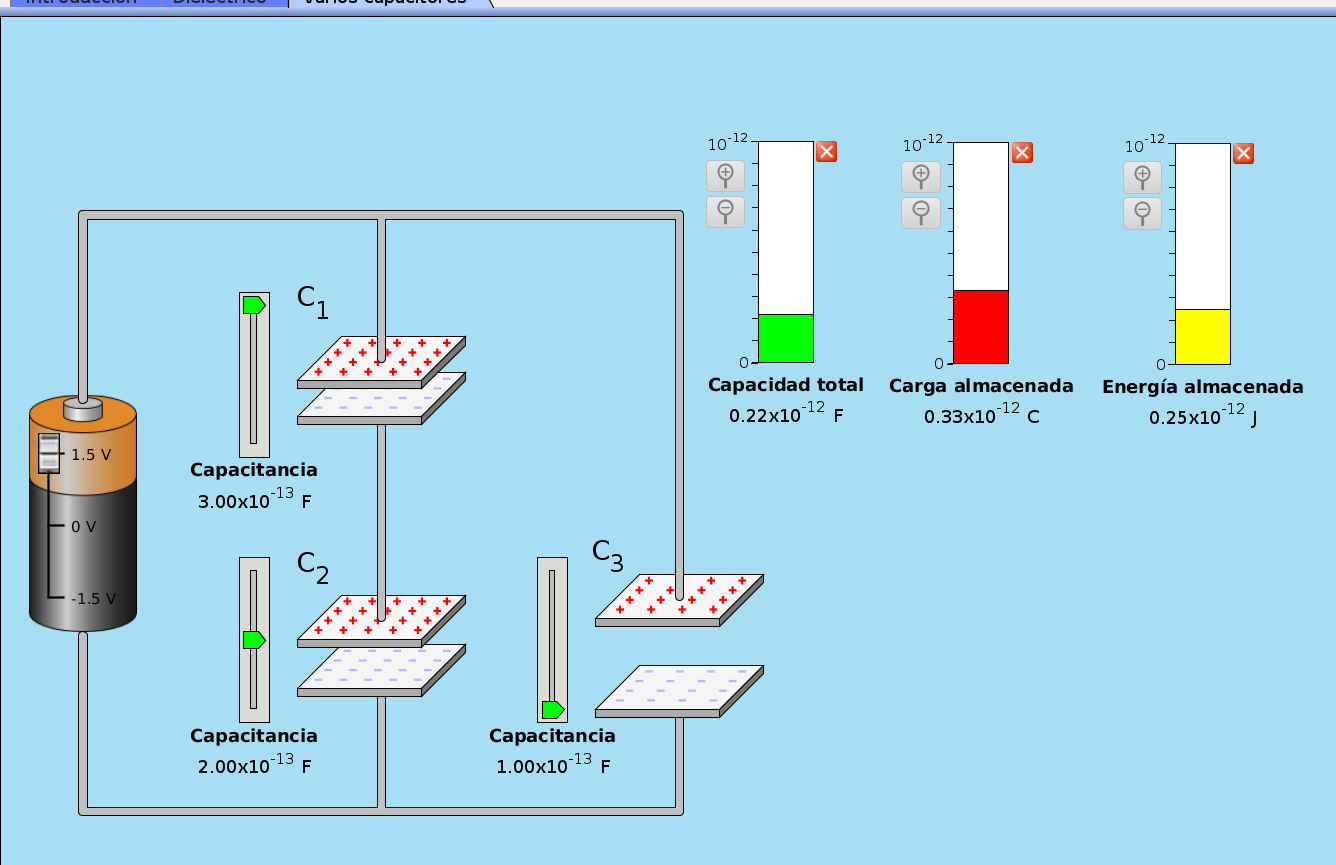
\includegraphics[width=0.9\textwidth]{./images/foto2ejercicio3Conexiondecapacitores.png}
\end{figure}



\end{enumerate}

\end{document}

